\section{Diskussion}
\label{sec:Diskussion}

% \subsection{Diskussion der Fehler}
% In der Theorie werden ideale Komponenten angenommen.
% Zur Berücksichtigung, dass eine reale Spule eine nicht zu vernachlässigende Induktivität $C_\text{Sp}$ aufweist, wird für die Auswertung angepasste Gesamtkapazitäten betrachtet.
% \begin{figure}
% 	\centering
% 	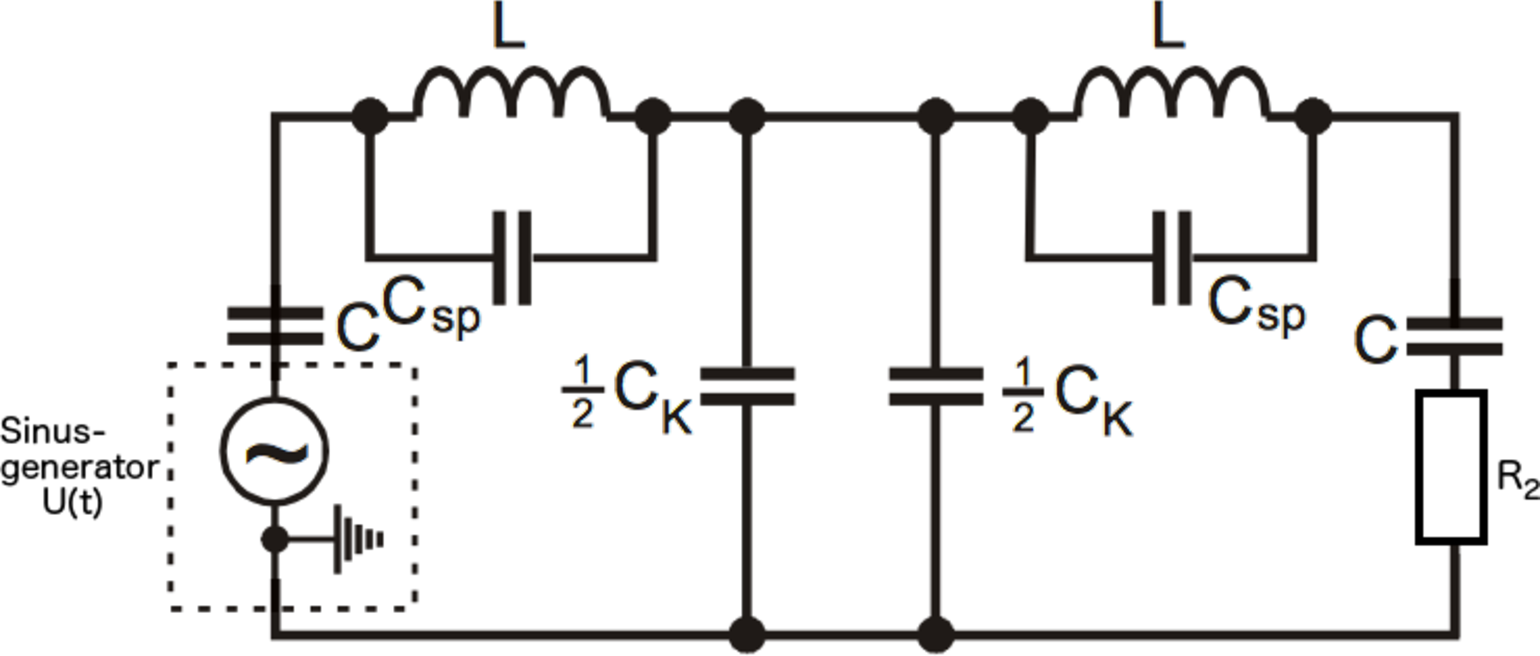
\includegraphics[width=0.5\textwidth]{Bilder/Auswertungsaufbau.pdf}
% 	\caption{Ersatzschaltung für die Auswertung. \cite{v355}}
% \end{figure}

% Für die Berechnung der Fundamentalfrequenz $f_+$ wird die Gesamtkapazität $C=C+C_\text{Sp.}$, für die Fundamentalfrequenz $f_-$ wird die Gesamtkapazität $C=(\frac{1}{C}+\frac{1}{C_\text{K}})^{-1}+C_\text{Sp.}$ betrachtet.

% \subsection{}
Für die Untersuchung von gekoppelten Schwingungen eignen sich elektrische Schaltungen sehr gut.
Die theoretischen Überlegungen gelten analog für andere gekoppelte Schwinger, etwa für mechanische Systeme.
Besondere Eignung zeigt die elektrische Schaltung dadurch, dass es mithilfe eines Oszilloskopes und eines Signalgenerators präzise ausgemessen werden kann.
Die konsequent geringen Abweichungen von Messung und Erwartungswert beweisen die Theorie und die Eignung der elektrischen Schaltung.
